\documentclass{article}
\usepackage{graphicx} % Required for inserting images
\usepackage{subcaption}
\graphicspath{{../simulations/}}
\begin{document}
\section{Bandgap Reference}
\begin{figure}[htbp]
    \centering
    % Left Subfigure
    \begin{subfigure}[b]{0.48\linewidth}
        \centering
        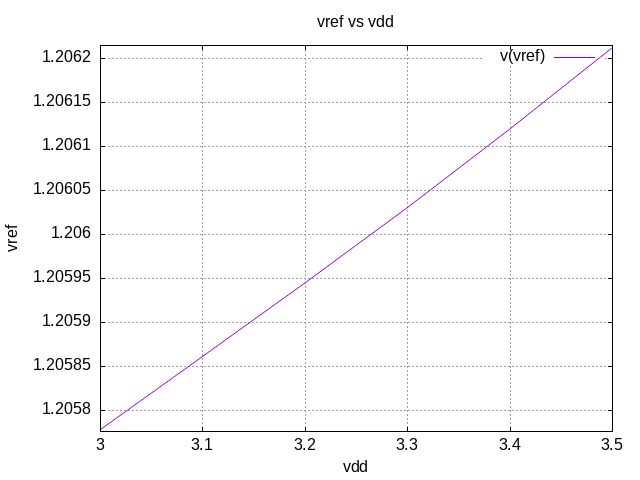
\includegraphics[width=\linewidth]{bandgap_vref_vs_vdd}
        \caption{Bandgap Vref vs VDD}
        \label{fig:tran}
    \end{subfigure}
    \hfill % Pushes the two figures apart
    % Right Subfigure
    \begin{subfigure}[b]{0.48\linewidth}
        \centering
        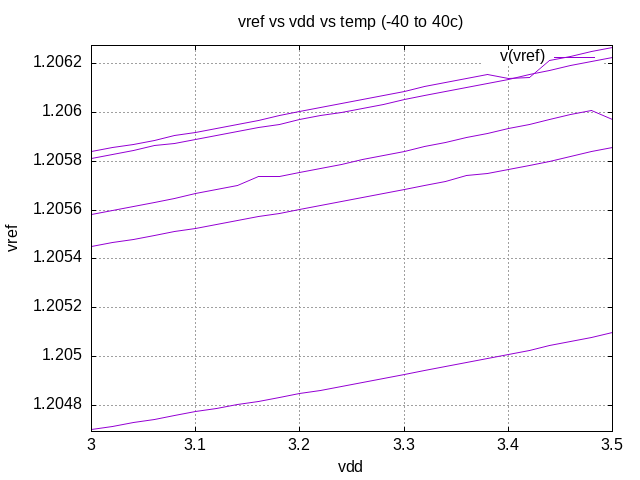
\includegraphics[width=\linewidth]{bandgap_vref_vs_vdd_vs_temp}
        \caption{Bandgap Vref vs VDD and Temperature}
        \label{fig:ac}
    \end{subfigure}
\end{figure}
\section{Opamp}
\begin{figure}[htbp]
    \centering
    % Left Subfigure
    \begin{subfigure}[b]{0.48\linewidth}
        \centering
        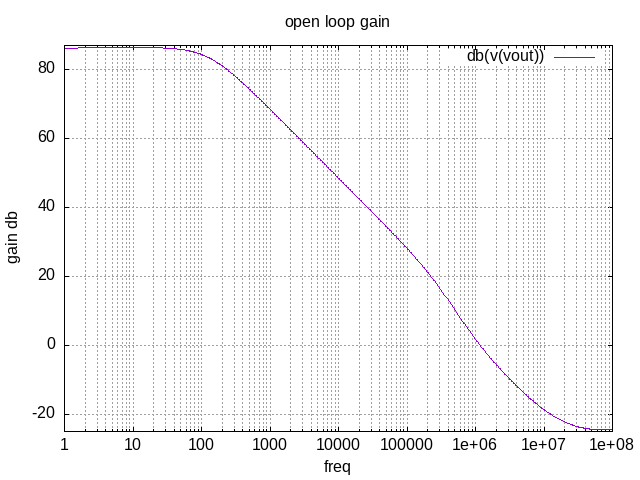
\includegraphics[width=\linewidth]{opamp_ac_mag}
        \caption{Opamp open loop gain}
        \label{fig:tran}
    \end{subfigure}
    \hfill % Pushes the two figures apart
    % Right Subfigure
    \begin{subfigure}[b]{0.48\linewidth}
        \centering
        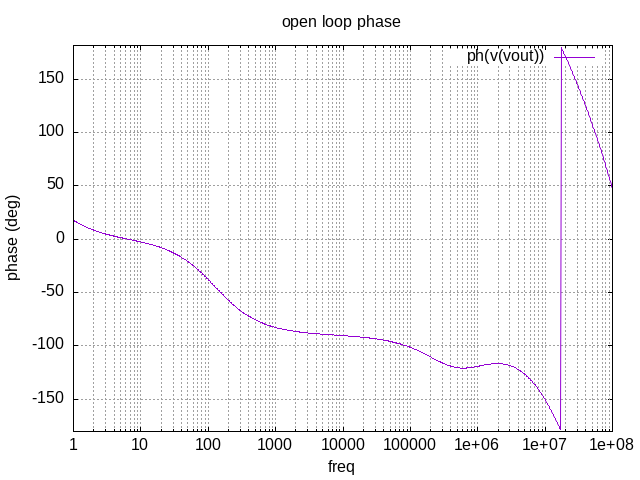
\includegraphics[width=\linewidth]{opamp_ac_phase}
        \caption{Opamp open loop phase}
        \label{fig:ac}
    \end{subfigure}
\end{figure}
\begin{figure}[htbp]
    \centering
    % Left Subfigure
    \begin{subfigure}[b]{0.48\linewidth}
        \centering
        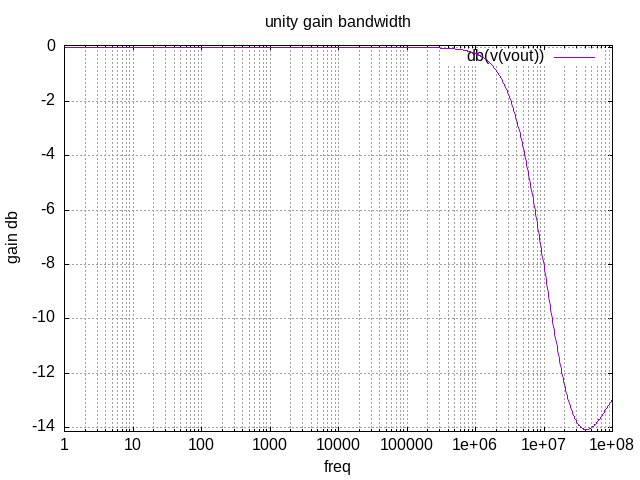
\includegraphics[width=\linewidth]{opamp_unity_gain}
        \caption{Opamp unity gain bandwidth}
        \label{fig:tran}
    \end{subfigure}
    \hfill % Pushes the two figures apart
    % Right Subfigure
    \begin{subfigure}[b]{0.48\linewidth}
        \centering
        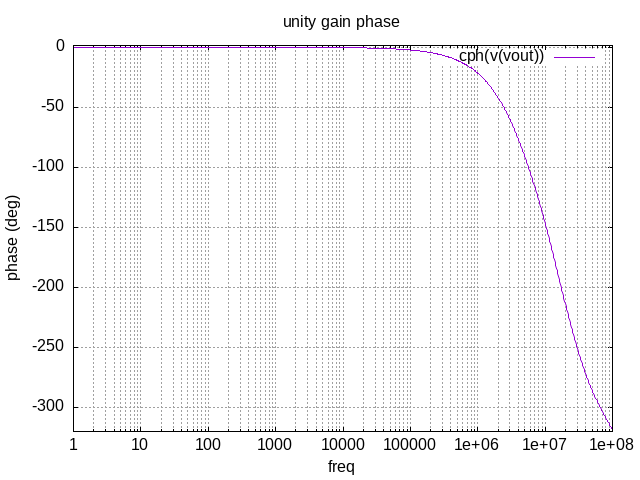
\includegraphics[width=\linewidth]{opamp_unity_gain_phase}
        \caption{Opamp unity gain phase}
        \label{fig:ac}
    \end{subfigure}
\end{figure}
\section{Instrumentaion Amp}
\begin{figure}[htbp]
    % Left Subfigure
    \begin{subfigure}[b]{0.48\linewidth}
        \centering
        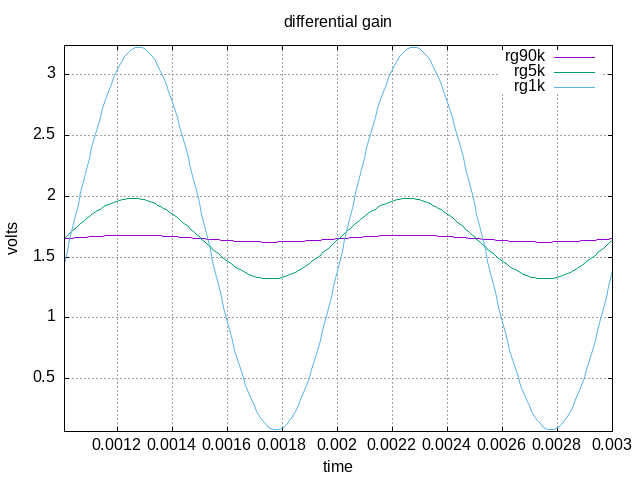
\includegraphics[width=\linewidth]{tran}
        \caption{Transisent response}
        \label{fig:tran}
    \end{subfigure}
    \hfill % Pushes the two figures apart
    % Right Subfigure
    \begin{subfigure}[b]{0.48\linewidth}
        \centering
        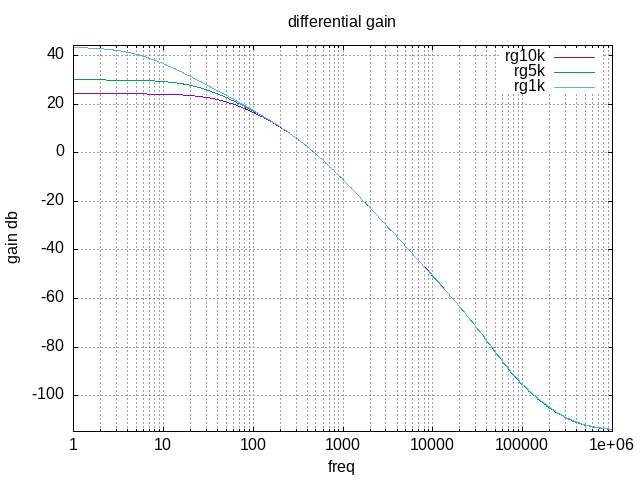
\includegraphics[width=\linewidth]{ac}
        \caption{Gain vs. Frequency}
        \label{fig:ac}
    \end{subfigure}
\end{figure}
\begin{figure}[htbp]
    \centering
    % Left Subfigure
    \begin{subfigure}[b]{0.48\linewidth}
        \centering
        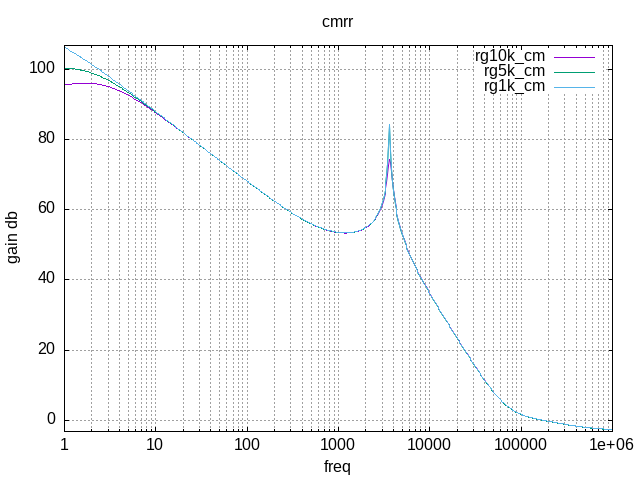
\includegraphics[width=\linewidth]{cmrr}
        \caption{CMRR vs Frequency}
        \label{fig:cmrr}
    \end{subfigure}
    \hfill % Pushes the two figures apart
    % Right Subfigure
    \begin{subfigure}[b]{0.48\linewidth}
        \centering
	    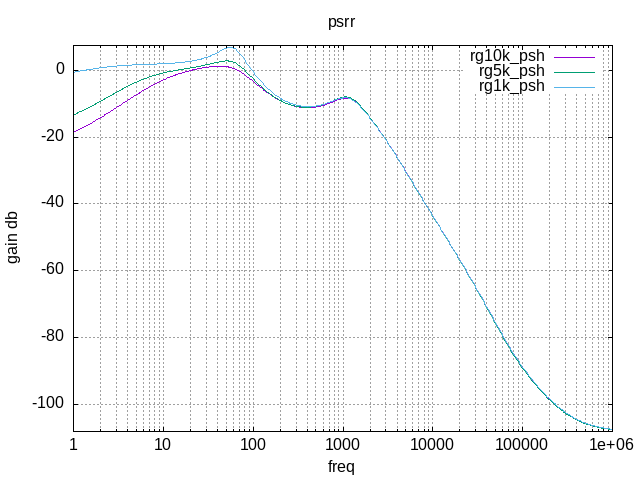
\includegraphics[width=\linewidth]{psrr}
        \caption{PSRR (high) vs Frequency}
        \label{fig:psrr}
    \end{subfigure}
\end{figure}
\end{document}
